% Created 2018-05-11 Fri 23:03
\documentclass[11pt]{article}
\usepackage[utf8]{inputenc}
\usepackage[T1]{fontenc}
\usepackage{fixltx2e}
\usepackage{graphicx}
\usepackage{longtable}
\usepackage{float}
\usepackage{wrapfig}
\usepackage{rotating}
\usepackage[normalem]{ulem}
\usepackage{amsmath}
\usepackage{textcomp}
\usepackage{marvosym}
\usepackage{wasysym}
\usepackage{amssymb}
\usepackage{hyperref}
\tolerance=1000
\author{thecsw}
\date{\today}
\title{u/prequelmemes$_{\text{bot}}$ Documentation}
\hypersetup{
  pdfkeywords={},
  pdfsubject={},
  pdfcreator={Emacs 25.3.1 (Org mode 8.2.10)}}
\begin{document}

\maketitle
\tableofcontents

\newpage
\textbf{Hello there!}

Welcome to the source page of u/prequelmemes$_{\text{bot}}$! Nice to meet you. First of
all, let me talk you through what the bot does and details later. \textbf{If you want}
to help the bot, please go down to the \textbf{TODO} list and find your way to
contribute! \emph{Thanks!}

\begin{figure}[htb]
\centering
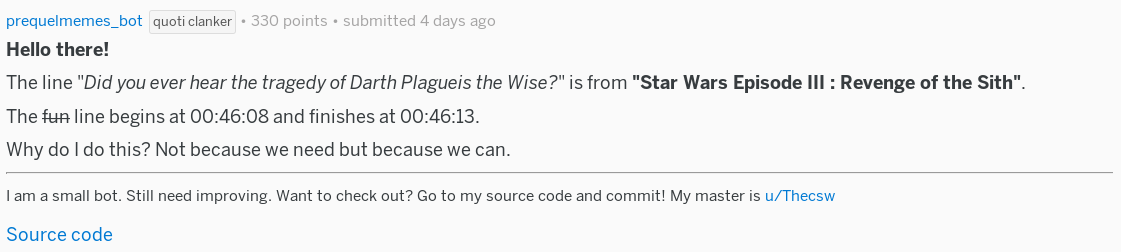
\includegraphics[width=.9\linewidth]{./doc/pic.png}
\caption{\label{preq_pic}A comment picture.}
\end{figure}

\section{Getting started}
\label{sec-1}

These instructions will get you a copy of the project up and running on your
local machine for development and testing purposes. See deployment for notes on
how to deploy the project on a live system. 

\subsection{Prerequisites}
\label{sec-1-1}

\begin{verbatim}
sudo pip install praw
sudo pip install python-opencv
sudo pip install pytesseract
sudo pip install tesseract-ocr
sudo pip install Pillow
sudo pip install tqdm
\end{verbatim}

OR

\begin{verbatim}
pip install --upgrade -r requirements.txt
\end{verbatim}
\begin{enumerate}
\item \href{https://github.com/praw-dev/praw}{praw} is Python Reddit API Wrapper. This will be the main and only package to
connect to Reddit's API and extract desired data.
\item \href{https://pypi.python.org/pypi/opencv-python}{python-opencv} is used for image transformations and computer vision problems.
\item \href{https://pypi.python.org/pypi/pytesseract}{pytesseract} is a python wrapper for Google's Tesseract-OCR.
\item \href{https://pillow.readthedocs.io/en/latest/}{Pillow} is the Python  Imaging Library by Fredrik Lundh and Contributors.
\item \href{https://pypi.python.org/pypi/tqdm}{tqdm} is used for fancy progress bars.
\end{enumerate}

\subsection{Other Dependencies}
\label{sec-1-2}

Tesseract engine should be installed on a local machine to run the text
recognition properly. We will also install the tesseract OCR trained 
languages for better accuracy and we will install only the English 
packages. For more information about other languages, please refer to 
tesseract's official 
\href{https://github.com/tesseract-ocr/tesseract}{repository on Github}.

\subsubsection{Linux}
\label{sec-1-2-1}

\begin{enumerate}
\item Debian, Ubuntu (aptitude)
\label{sec-1-2-1-1}

\begin{verbatim}
sudo apt-get install tesseract-ocr
sudo apt-get install tesseract-ocr-eng
\end{verbatim}

\item Arch Linux (pacman)
\label{sec-1-2-1-2}

\begin{verbatim}
sudo pacman -S tesseract
sudo pacman -S tesseract-data-eng
\end{verbatim}
\end{enumerate}

\subsubsection{Mac OS (homebrew)}
\label{sec-1-2-2}
\begin{verbatim}
brew install tesseract
\end{verbatim}

\section{Installing}
\label{sec-2}

The only thing that needs to be done before execution is the config. The only
thing that needs to be done before execution is the config profile. In the
config profile you should fill your Reddit API details.

For that please follow the steps below

\begin{verbatim}
git clone https://github.com/thecsw/prequelmemes_bot
cd prequelmemes_bot
mv example.config.py config.py
nano config.py
\end{verbatim}

After filling out the details, save and exit. You're done with installation.

\section{Deployment}
\label{sec-3}

Remove the word \textbf{*'example'*} from the title of all files with it.

Just run this

\begin{verbatim}
python main.py
\end{verbatim}

That is everything. All the prequelmemes will be identified. Once and for all,
the archives will never be incomplete.

\section{Source code}
\label{sec-4}

The code is heavily commented and all the important modules are being separated
into different files. Looks pretty, dunno.

\section{Built With}
\label{sec-5}
\begin{enumerate}
\item \href{https://github.com/praw-dev/praw}{praw} is Python Reddit API Wrapper. This will be the main and only package to
connect to Reddit's API and extract desired data.
\item \href{https://pypi.python.org/pypi/opencv-python}{python-opencv} is used for image transformations and computer vision problems.
\item \href{https://pypi.python.org/pypi/pytesseract}{pytesseract} is a python wrapper for Google's Tesseract-OCR.
\item \href{https://pypi.python.org/pypi/tqdm}{tqdm} is used for fancy progress bars.
\item \href{https://pillow.readthedocs.io/en/latest/}{Pillow} is the Python  Imaging Library by Fredrik Lundh and Contributors.
\end{enumerate}

\section{Authors}
\label{sec-6}
\begin{itemize}
\item \textbf{Sagindyk Urazayev} - \emph{Initial work} - \href{https://github.com/thecsw}{thecsw}
\item \textbf{farhank3389} - \emph{Fixes} - \href{https://github.com/farhank3389}{farhank3389}
\end{itemize}
\section{License}
\label{sec-7}

This project is licensed under the The GNU General Public License (see the
\href{https://github.com/thecsw/prequelmemes_bot/blob/master/LICENSE}{LICENSE.md} file for details), it explains everything pretty well. 

\section{Todo list}
\label{sec-8}

This is going to be a short todo list. If you have the true loyalty and some
free time, try to add/fix the following todo items or add your own with the
issues tab or push.

\subsection{{\bfseries\sffamily TODO} Edit the mesage body text.}
\label{sec-8-1}

The message body text isn't perfect. It can be more prequelmemed. So yeah, if
somebody can do it, that would be awesome.

\subsection{{\bfseries\sffamily TODO} Port the code to python3.6+}
\label{sec-8-2}

Just port the whole code. I am not talking about just using \verb~python3 main.py~
instead of \verb~python main.py~. I am talking about using the new python3+
features. Like better string formatting, like the \verb~print(f"{args}...")~.

\subsection{{\bfseries\sffamily TODO} Get rid of the tqdm.}
\label{sec-8-3}

I don't know whym but tqdm has been throwing some errors at me. I should replace
it with some \textbf{manual} loop counter. We are talking CS101 here. Heh

\subsection{{\bfseries\sffamily TODO} Make some general fixes to the code.}
\label{sec-8-4}

Add some little new features, replace old ones with new ones. Make a faster
version. Just a general quality assurance.

\subsection{{\bfseries\sffamily TODO} Add a comment feature.}
\label{sec-8-5}

I don't have an idea of what to do. I made some prototypes, don't know. If the
bot is going to answer to each comment, that is just a spam.
% Emacs 25.3.1 (Org mode 8.2.10)
\end{document}